\textbf{Problem 4.}

Let us once solve the Poisson equation:
\begin{align*}
    -u_{xx} = f(x), \quad \text{for} \quad x\in(0,1)
\end{align*}

but this time with boundary conditions $u(0)=0$ and $u_x(1) = -2e$, numerically using a 2nd order central difference approximation and a uniform grid of size $\Delta x$.  We wish to study the accuracy of the numerical scheme and the order of convergence of the solution using the modified norm $\norm{\cdot}_2^*$.  Our function $f(x)$ is given as
\begin{align*}
    f(x) = (6x + 2x^2)e^x
\end{align*}

We can impose the boundary condition $u_x(1) = -2e$ via two methods:
\begin{enumerate}[label=(\alph*),itemsep=0mm]
    
    \item First-order backward different approximation for the derivative
    \item Second-order central difference approximation for the derivative
    
\end{enumerate}

We plot the results in Fig. \ref{hw2_qn4}.

\begin{figure*}[h!]
\centering
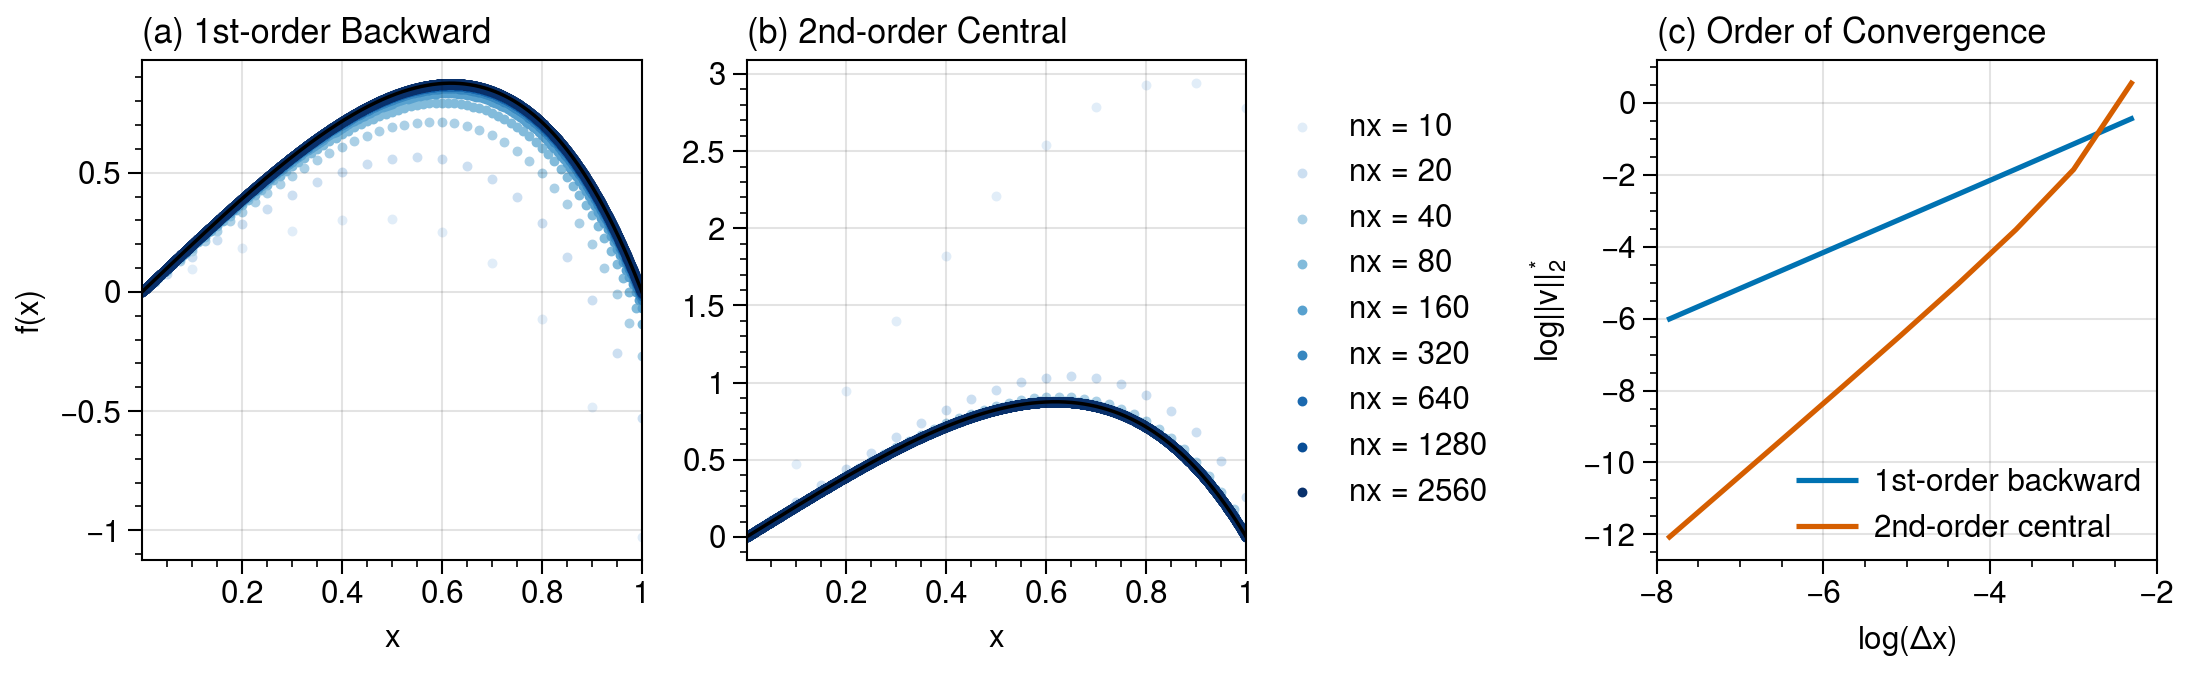
\includegraphics[width=\textwidth]{figures/hw2_qn4_numericalsol.png}\\
\caption{Plots of the numerical solutions for (a) 1st-order backward and (b) 2nd-order central difference approximations for the derivative, with (c) showing the rate of convergence for the two methods}
\label{hw2_qn4}
\end{figure*}

We see that method (a) has 1st order convergence, while (b) has a 2nd order convergence.  This is made explicit when plotting $\norm{\cdot}_2^*$ against $\Delta x$, where we see that $\norm{\cdot}_2^*$ decreases much more sharply for method (b) than for method (a) as $\Delta x \rightarrow 0$.